\textit{To relate the datasets it is necessary to identify links among them. In this chapter, we discuss how linking entries across heterogeneous data sources such as databases or knowledge bases, which becomes an increasingly difficult problem, in particular w.r.t. the runtime of these tasks. 
Consequently, it is of utmost importance to provide time-efficient approaches for similarity joins in the Web of Data. 
While a number of scalable approaches have been developed for various measures, the Most Frequent $k$ Characters (MFKC) measure has not been tackled in previous works. 
We hence present a sequence of filters that allow discarding comparisons when executing bounded similarity computations without losing recall. 
Therewith, we can reduce the runtime of bounded similarity computations by approximately 70\%.  
Our experiments with a single-threaded, a parallel and a GPU implementation of our filters suggest that our approach scales well even when dealing with millions of potential comparisons.}

\section{Introduction}
The problem of managing heterogeneity at both the semantic and syntactic levels among various information resources \cite{valdestilhasdbpediasameas,shvaiko2013ontology} is one of the most difficult problems on the information age.
%This problem is even harder to tackle when these information resources are always growing up. 
This is substantiated by most of the database research self-assessment reports, which acknowledge that the hard question of semantic heterogeneity, that is of handling variations in meaning or ambiguity in entity interpretation, remains open \cite{shvaiko2013ontology}. In knowledge bases, Ontology Matching (OM) solutions address the semantic heterogeneity problem in two steps: (1) matching entities to determine an alignment, i.e., a set of correspondences, and (2) interpreting an alignment according to application needs, such as data translation or query answering. Record Linkage (RL) and, more recently, Link Discovery\footnote{The expression "link discovery" in this paper means the discovery of typed relations that link instances from knowledge bases on the Web of Data. We never use it in the sense of graph theory.} (LD) solutions on the other hand aim to determine pairs of entries that abide by a given relation $R$. In both cases, string similarities are used  to compute candidates for alignments. %Therewith, providing interoperability to the Semantic Web and a tool in some classical data integration tasks dealing with the Semantic Web heterogeneity problem. The ontologies are used as input and works determining as output a set of correspondences between the semantically related entities of those ontologies. 
In addition to being central to RL and LD, these similarities also play a key role in several other tasks such as data translation, ontology merging and navigation on the Web of Data \cite{shvaiko2013ontology,euzenat2007ontology}.

One of the core tasks when developing time-efficient RL and LD solutions hence lies in the development of time-efficient string similarities. 
%In particular, the string similarity is located on the matching step, where we develop an improvement on the state of the art, also we assume as the naive approach of the Most Frequent K Characters (MFKC) \cite{seker2014novel} that will be covered in this paper.
In this paper, we study the MFKC similarity function \cite{seker2014novel} and present an approach for improving the performance of similarity joins.
To this end, we develop a series of filters which guarantee that particular pairs of resources do not abide by their respective similarity threshold by virtue of their properties.
% We explain our approach by using an example from link discovery based on the data shown in \Cref{example}.
% Here, the task is to detect candidates for pairs $(s, t) \in \ds{} \times \dt{}$ such that $s \approx t$,
% where $\ds{}$ and $\dt{}$ are two datasets and $\approx$ means \textit{same entity as}.

%In this paper, we address an efficient execution of the MFKC as a string similarity measure using a threshold and filters in order to discard unnecessary computations.

The contributions of this paper are as follows:

\begin{enumerate}
	%	\item The performance (run-time) was improved and outperforms the naive approach \cite{seker2014novel}.
	
	\item We present two nested filters, (1) First Frequency Filter and (2) Hash Intersection filter, that allow to discard candidates before calculating the actual similarity value, thus giving a considerable performance gain.
	
	\item We present the \emph{k similarity filter} that allows detecting whether two strings $s$ and $t$ are similar in a fewer number of steps. 
	%with the possibility to give the final satisfactory similarity score before process all k characters, thus, improving the performance.
	
	% according our Most Frequent K Character algorithm. 
	
	\item We evaluate our approach with respect to its runtime and
	its scalability with several threshold settings and
	dataset sizes.%, also to show that our approach fixes some problems. 
	
	\item We present several parallel implementations of our approach and show that they work well on problems where $|\ds{} \times \dt{}| \geq 10^5$ pairs. 
	%also outperform JaroWinkler \cite{winkler1990string}.
\end{enumerate}

The rest of the chapter is structured as follows: 
% In \Cref{preliminaries} we present the preliminaries, including the formal notation necessary to understand our work and the naive approach. 
In section \ref{mfkc}, we present our nested filters that allow reducing the runtime of the MFKC similarity joins. We then evaluate our approach in section \ref{evaluation}, where we focus on approaches that aim to improve the time-efficiency of the link discovery task. 

%\section{Preliminaries} \label{preliminaries}

%Three types of text similarity are commonly used in literature \cite{gomaa2013survey}: 
%(1) String-based similarities operate on string sequences and character composition, where a string metric measures similarity or dissimilarity (distance) between two text strings for approximate string matching or comparison. (2) Corpus-based similarity are similarity measures that compute the similarity of words by means of information gained from large corpora. Finally, (3) Knowledge-based similarities are semantic similarity measures that are based on the identification of the degree of similarity between words using information derived from semantic networks.

%We study a string-based similarity, the k most frequent common characters. Let $\sum$ be an alphabet and $\sum^*$ be the set all sequences that can be generated by using elements of $\sum$. We call the elements of $\sum$ characters and assume that $\sum$ contains the empty character $\epsilon$.

%The formal specification of link discovery adopted herein is equivalent
%to the definition proposed in \cite{ngomo2012link}: Given a set $\ds{}$ of
%source resources, a set $\dt{}$ of target resources and a relation $R$, our goal is to find the set $M \subseteq \ds{} \times \dt{}$ of pairs
%$(s, t)$ such that $R(s, t)$. If $R$ is \aurl{owl}{sameAs}, then we
%are faced with a deduplication task. Given that the explicit computation of $M$ is usually a very complex endeavor, 
%$M$ is most commonly approximated by a set
%$M' = \{(s, t, \upsigma(s, t)) \in \ds{} \times \dt{} \times \mathbb{R}^+ : \upsigma(s, t) \geq \theta\}$,
%where $\upsigma$ is a similarity function
%and $\theta \in [0, 1]$ is a similarity threshold. Given that this problem is in $O(n^2)$, using naive algorithms to compare large $\ds{}$ %and $\dt{}$ is most commonly impracticable.
%Thus, time-efficient approaches for the computation of bounded measures have been developed over the last years for measures such as the Levenshtein distance, Minkowski distances, trigrams and many more \cite{ngomo2012min}.

\section{Approach} \label{mfkc}

Let us call $NaiveMFKC$ the function which computes the MFKC algorithm as described in \cite{seker2014novel}.
Such function works with three parameters, i.e. two strings $s$ and $t$ and an integer $lim$ and returns the sum of frequencies, where $\f{c_i, s}$ is a function that returns the frequency of the character $c_i$ in the string $s$ and $s \supseteq \{c_1,...,c_n\}$, i.e $\f{a,"andrea"}=2$, because the character $a$ has been found twice and the hash functions $h(s)$ and $h(t)$ containing the characters and their frequencies. The output of function is always positive, as shown in equation \ref{eq:naive}. 
%Hence, its definition is the following:
\begin{equation} \label{eq:naive}
	NaiveMFKC(s, t, lim) = lim - \sum_{c_i \in h(s) \cap h(t)}^2 f(c_i,s) + f(c_i,t)
\end{equation}
%where the hash functions $h(s)$ and $h(t)$ contain characters and their frequencies.

Our work aims to reduce the runtime of computation of the MFKC similarity function.
Here, we use a sequence of filters, which allow discarding similarity computations and imply in a reduction of runtime.
As input, the algorithm receives datasets $\ds{}$ and $\dt{}$, an integer number representing the $k$ most frequent characters and a threshold $\theta \in [0,1]$.
The similarity score of the pair of strings from the Cartesian product from $\ds{}$ and $\dt{}$ must have a score greater or equal the threshold $\theta$ to be considered a good pair, i.e. 
for a given threshold $\theta$, if the similarity function has a pair of strings with similarity score less than the threshold, $\sigma (s, t) < \theta$, we can discard the computation of the MFKC score for this pair. Our final result is a set which contains the pairs having similarity score greater than or equal to the threshold, i.e. $\sigma(s,t) \geq \theta$.

% \begin{table}[H]
% 	\centering
% 	\caption{Example data sets. Sources (\ds{}) and Targets (\dt{})}
% 	\begin{tabular}{llll}
% 		\hline\noalign{\smallskip}
% 		\textbf{id} & \textbf{Content} & \textbf{id} & \textbf{Content} \\
% 		\noalign{\smallskip}
% 		\hline
% 		\noalign{\smallskip}
% 		s1 & Wari culture & t1 & Wari culture \\ 
% 		s2 & Chrabrany & t2 & Chrabrany \\ 
% 		s3 & Accum & t3 & Accum \\ 
% 		s4 & Jaintia Kingdom & t4 & Kingdom of Kano \\ 
% 		s5 & Dominion of Melchizedek & t5 & Dominion of Melchizedek \\
% 		\hline
% 	\end{tabular}
% 	\label{example}
% \end{table}

Our work studies the following problem:
Given a threshold $\theta \in [0, 1]$ and two sets of strings
$\ds{}$ and $\dt{}$, compute the set $M' = \{(s, t, \upsigma(s, t)) \in
\ds{} \times \dt{} \times \mathbb{R}^+ : \upsigma(s, t) \geq \theta\}$. 
Two categories of approaches can be considered to improve the runtime of measures: 
Lossy approaches return a subset $M''$ of $M'$ which can be calculated efficiently but for which there are no guarantees that $M'' = M'$. 
Lossless approaches, on the other hand, ensure that their result set $M''$ is exactly the same as $M'$.
In this paper, we present a lossless approach that targets the MFKC algorithm. 
% \subsection{A High-Performance Approach to String Similarity using Most Frequent K Characters} \label{newMFKC}
% Here we will work with an extension of the state of the art \cite{seker2014novel} in order to cover all possible $K$ characters, not only two as stated in the original approach. We also include a threshold $\theta$ and a similarity score normalized between values from 0 to 1.
Equation \ref{eq:1} shows our definition for the string similarity function $\upsigma$ for the MFKC.
\begin{equation} \label{eq:1}
	\upsigma(s,t)=
	\frac
	{\sum_{c_i \in h(s,k) \cap h(t,k)} \f{c_i,s}+\f{c_i,t}}
	{|s|+|t|}
\end{equation}
where $s$ and $t$ are strings, such that $s,t \in \sum^*$, $\f{c_i, s}$ is a function that returns the frequency of the character $c_i$ in the string $s$, where $s \supseteq \{c_1,...,c_n\}$, $k$ represents the limitation of the elements that belongs to the hashes; set $h(s,k) \cap h(t,k)$ means the intersection between the keys of hashes $h(s,k)$ and $h(t,k)$ (i.e., the most frequent K characters).
% Viewing hashes as data structures, we have:
% \noindent $
% e=\langle e_c, e_f \rangle \\
% \h{s}=\{e_i|e_i.c \in s, e_i.f=freq(c,s)  \} \\
% e_i.f \geq e_{i+1}.f \\
% (e_i.f = e_{i+1}.f) \Rightarrow e_i.c < e_{i+1}.c
% $
% 
% \noindent The keys are the characters and the values are the respective frequencies.
We expect two steps to obtain the similarity score:
\begin{enumerate}
	\item Firstly, we transform the strings $s$ and $t$ in two hashes using Most Frequent Character Hashing \cite{seker2014novel}, according to the following example with $k=3$:
	
	$s=aabbbcc \ \rightarrow \ \h{s,k}=\{b=3,a=2,c=2\} \\
	t=bbccddee \ \rightarrow \ \h{t,k}=\{b=2,c=2,d=2\}$
	
	\item We calculate the sum of the character frequencies of matching characters on the hashes $h(s,k)$ and $h(t,k)$, then, we normalize dividing by the sum of the length of $|s|$ and $|t|$ resulting in a similarity score from $0$ to $1$ according to the equation \ref{eq:d1} and the resulting score should be greater or equals the threshold $\theta$.
	\begin{equation} \label{eq:d1}
		\upsigma(s,t,k,\theta) = \frac{\sum_{c_i \in \h{s,k} \cap \h{t,k}} \f{c_i,s}+\f{c_i,t}}{|s|+|t|} \geq \theta
	\end{equation}
	
\end{enumerate}

\subsection{Improving the Runtime}

%In this section the runtime of the Most Frequent K Characters, already defined at \Cref{eq:1}, is improved using a heuristic technique, that here is called filters.

In this section, the runtime of MFKC defined in equation \ref{eq:1} is improved using filters where $\mathcal{N}$ is the output of first frequency filter, $\mathcal{L}$ is the output of hash intersection filter and $\mathcal{A}$ represents the output of the $k$ similarity filter. 

\subsubsection{First Frequency Filter} \label{fff}

As specified in the definition of MFKC \cite{seker2014novel} this filter assumes that the hashes are already sorted in an descending way according to the frequencies of characters, therefore the first element of each hash has the highest frequency.

\begin{theorem} \label{thr:ff1}
Showing that:
\begin{equation} \label{eq:ff1}
	\sigma(s,t)= \frac
	{\sum_{c_i \in \h{s,k} \cap \h{t,k}} \f{c_i,s}+\f{c_i,t}}
	{|s|+|t|} \leq \frac{h_1(s,k) k + |t|}{|s| + |t|}
\end{equation}
implies that $\sigma(s,t) < \theta$.
\end{theorem}

% \noindent where $h_1(s,k)$ means the frequency of first element of the hash $h(s,k)$. For example, the $h(s,k)=\{b=3,a=1,d=1\}$, then $h_1(s,k)=\{3\}$. Therefore, once we have 
% \begin{equation} \label{eq:ff0}
% 	\frac{h_1(s,k) k + |t|}{|s| + |t|} < \theta,
% \end{equation}
% \noindent the pair of strings $s$ and $t$ can be discarded without calculating the entire similarity.

\begin{proof}[Theorem \ref{thr:ff1}]
	Let the intersection between hashes $h(t,k)$ and $h(s,k)$ be a set of characters from $c_1$ to $c_n$, such that equation \ref{eq:intersection}: 
	\begin{equation} \label{eq:intersection}
	h(t,k) \cap h(s,k)=\{c_1,...,c_n\}
	\end{equation}
	According to the definition of the frequencies $\f(c_i, t)$ we have equation \ref{eq:tsub}: 
	\begin{equation} \label{eq:tsub}
	t \supseteq \{c_1,...,c_1,...,c_n,...c_n\}
	\end{equation}
	where each $c_i$ appears $\f(c_i,t)$ times,  
	therefore: 
	\begin{equation} \label{eq:proof1}
	\f(c_1,t) + ... + \f(c_n, t) \leq |t|
	\end{equation}
	
	\noindent	Also, as $n \leq k$, because $t \supseteq \{c_1,...,c_n\}$, and $\f(c_i,s) \leq h_1(s,k)~ \forall_ {i=1,...,n}$, then: 
	\begin{equation} \label{eq:proof2}
	\begin{split}
	\f(c_1,s) + ... + \f(c_n,s) \leq h_1(s,k) + ... + h_1(s,k)
	=n (k) \leq k (h_1(s,k))
	\end{split}
	\end{equation}
	
	Therefore, from equation \ref{eq:proof1} and equation \ref{eq:proof2}, we obtain the equation \ref{eq:obt1}:
	
	\begin{equation} \label{eq:obt1}
	\begin{split}
	\frac
	{\sum_{c_i \in \h{s,k} \cap \h{t,k}} \f{c_i,s}+\f{c_i,t}}
	{|s|+|t|}
	=\frac
	{\sum_{i=1}^n \f(c_i,t) + \sum_{i=1}^n \f(c_i,s)}
	{|s|+|t|}
	\leq \frac{h_1(s,k) k + |t|}{|s| + |t|} 
	\end{split}
	\end{equation}

% Using examples from \Cref{example}, let us assume $\theta=1.0$ and $\ds{}.content$ has been mapped to $\dt{}.content$, then at the end of this step,
% 5 of the 25 initial pairs in $\ds{} \times \dt{}$ are dismissed. The remaining 20 pairs are:

% % skiped s1,t3 and s5,t3.

% $\mathcal{N}=\{ 
% \langle s1,t1 \rangle, \langle s1,t2 \rangle, \langle s1,t4 \rangle, \langle s1,t5 \rangle, 
% \langle s2,t1 \rangle, \langle s2,t2 \rangle, \\  
% \langle s2,t4 \rangle, \langle s2,t5 \rangle, \langle s3,t1 \rangle, \langle s3,t2 \rangle, \langle s3,t3 \rangle, \langle s3,t4 \rangle, \langle s3,t5 \rangle, \\ \langle s4,t1 \rangle, \langle s4,t2 \rangle, \langle s4,t4 \rangle, \langle s4,t5 \rangle, \langle s5,t1 \rangle, \langle s5,t4 \rangle, \langle s5,t5 \rangle
% \}$

Consequently, the rule which the filter relies on is the following.

\begin{equation}
	\langle s,t \rangle \notin \mathcal{N} \Rightarrow \langle s,t \rangle \notin \ds{} \times \dt{} \wedge \frac{h_1(s,k) k + |t|}{|s|+|t|} \leq \theta 
\end{equation}
\end{proof}

\subsubsection{Hash Intersection Filter} \label{hashintfilter}
In this filter, we check if the intersection between two hashes is an empty set, then the MFKC, represented by $\upsigma$, will return a similarity score of 0 and we can avoid the computation of similarity in this case.
Consequently, the rule which the filter relies on is the following.

\begin{equation}
	\langle s,t \rangle \in \mathcal{L} \Rightarrow \langle s,t \rangle \in \ds{} \times \dt{} \wedge |h(s) \cap h(t)| > 0
\end{equation}

we also can say that the equation \ref{h:1} represents a valid implication.
\begin{equation} \label{h:1}
	h(s) \cap h(t) = \emptyset \Rightarrow \upsigma(s,t)=0
\end{equation}

The equation \ref{h:1} means that if the intersection between $h(s,k)$ and $h(t,k)$ is a empty set, this implies that the similarity score will be 0.
% A example using this filter is, given two strings \\ $s="aaabbbccc"$ and $t="dddeeew"$, the hashes will be $\h{s,k}=\{a=3,b=3,c=3\}$ and $\h{t,k}=\{d=3,e=3,w=1\}$ then there is no intersection between the keys of these hashes.
That means there is no character matching, then there is no need to compute the similarity for this pair of strings.

% Using examples from \Cref{example}, let us assume $\theta=1.0$ and $\ds{}.content$ has been mapped to $\dt{}.content$, then at the end of this step,
% 1 of the 20 pairs in $\ds{} \times \dt{}$ are dismissed. The remaining 19 pairs are:

% $\mathcal{L}=\{ 
% \langle s1,t1 \rangle, \langle s1,t2 \rangle, \langle s1,t4 \rangle, \langle s1,t5 \rangle, 
% \langle s2,t1 \rangle, \langle s2,t2 \rangle, \\ \langle s2,t4 \rangle, \langle s2,t5 \rangle,
% \langle s3,t1 \rangle, \langle s3,t3 \rangle, \langle s3,t4 \rangle, \langle s3,t5 \rangle, \langle s4,t1 \rangle, \\ \langle s4,t2 \rangle, \langle s4,t4 \rangle, \langle s4,t5 \rangle,
% \langle s5,t1 \rangle, \langle s5,t4 \rangle, \langle s5,t5 \rangle
% \}$

\subsubsection{K Similarity filter} \label{mfc:filter}

For all the pairs left, the similarity score among them is calculated. After that, the third filter selects the pairs whose similarity score is greater or equal than a threshold $\theta$. 

\begin{equation}
	\langle s,t \rangle \in \mathcal{A} \Leftrightarrow \langle s,t \rangle \in \mathcal{N} \wedge \upsigma(s,t) \geq \theta
\end{equation}

This filter provides a validation and we show that the score of previous $k$ similarity is always lower than the next $k$, according to the equation \ref{eq:m1} and in some cases when the similarity score is been reached before compute all elements $\in \h{s,k} \cap \h{t,k}$, thus saving computation in these cases. 

Here $k$ is also used as a index of similarity function $\sigma_k(s,t)$ in order to get the similarity of all cases of $k$, from 1 to $k$, also to show the monotonicity.

Therefore we can say that the computation of similarity score occurs until $\upsigma_k(s,t) \geq \theta$.

We will demonstrate that the similarity score of previous $k$ similarity is always lower than the next $k$ similarity, for all $k \in \mathbb{Z}^* : k \leq |s \cap t|$. 

\begin{equation}\label{eq:m1}
	\upsigma_{k+1}(s,t) \geq \upsigma_{k}(s,t)
\end{equation}

% As our \textbf{base case} we provide two strings $s="amoroso"$ and $t="amoras"$, the similarity score for the first 4 $k$ is $\upsigma_{k=1}(s,t)=0.30$, $\upsigma_{k=2}(s,t)=0.53$, $\upsigma_{k=3}(s,t)=0.69$, $\upsigma_{k=4}(s,t)=0.84$.

We rewrote the equation for the first iteration, according to equation \ref{eq:m2}

\begin{equation} \label{eq:m2}
	\upsigma_{k}(s,t)=\frac
	{\sum_{c_i \in \h{s,k} \cap \h{t,k}, i=1}^k \f{c_i,s}+\f{c_i,t}}
	{|s|+|t|}
\end{equation}

Let $k \in \mathbb{Z}_+$ be given and suppose the equation \ref{eq:m1} is true for $k+1$. %Then (see \Cref{eq:k1,eq:k2,eq:k3})

% \begin{equation} \label{eq:k1}
% 	\begin{split}
% 	\frac 
% 	{\sum_{c_i \in \h{s,k} \cap \h{t,k}}^{k+1} \f{c_i,s}+\f{c_i,t}}{|s|+|t|} \geq
% 	\frac
% 	{\sum_{c_i \in \h{s,k} \cap \h{t,k}}^{k} \f{c_i,s}+\f{c_i,t}}{|s|+|t|}
% 	\end{split}
% \end{equation}

% \begin{equation} \label{eq:k2}
% 	\begin{split}
% 	\sum_{c_i \in \h{s,k} \cap \h{t,k}}^{k+1} \f{c_i,s}+\f{c_i,t} \geq \sum_{c_i \in \h{s,k} \cap \h{t,k}}^k \f{c_i,s}+\f{c_i,t}
% 	\end{split}
% \end{equation}

\begin{equation} \label{eq:k3}
	\begin{split}
	\sum_{c_i \in \h{s,k} \cap \h{t,k}}^{k} \begin{bmatrix} \f{c_i,s}+\f{c_i,t}\end{bmatrix} + \f{c_{k+1},s}+\f{c_{k+1},t}
	\geq \sum_{c_i \in \h{s,k} \cap \h{t,k}}^k \f{c_i,s}+\f{c_i,t}
	\end{split}
\end{equation}

Therefore, we can notice that the sum of frequencies will be always greater or equal 0, according to $\f{c_{k+1},s}+\f{c_{k+1},t} \geq 0$. Thus, equation \ref{eq:m1} holds true.

% Using examples from \Cref{example}, let us assume $\theta=1.0$ and $\ds{}.content$ has been mapped to $\dt{}.content$, then at the end of this step, 15 of the 19 pairs in $\ds{} \times \dt{}$ are dismissed. The remaining 4 pairs are:

% $\mathcal{A}=\{ \langle s1,t1 \rangle, \langle s2,t2 \rangle, \langle s3,t3 \rangle, \langle s5,t5 \rangle \}$

\subsubsection{Filter sequence}

The sequence of the filters occurs basically in 4 steps, (1) We starting to make the Cartesian product with the pairs of strings from the datasets $\ds{}$ and $\dt{}$, (2) Discarding pairs using the $First~Frequency~Filter(\mathcal{N})$, (3) Discarding pairs where there is no matching characters with the $Hash~Intersection~filter (\mathcal{L})$ and (4) With the Most Frequent Character Filter $(\mathcal{A})$ we will process only similarities greater or equal the threshold $\theta$, if the similarity function $\upsigma(s,t) \geq \theta$ in the first k characters we can stop the computation of the similarity of this pair, saving computation and add to our dataset with resulting pairs $Dr$, also shown in the algorithm \ref{alg:1}.

% \begin{figure}[htb] 
% 	\centering
% 	\includegraphics[width=350pt]{img/filterseq4}
% 	\caption{Filter Sequence.}
% 	\label{fig:fs1}
% \end{figure}

\begin{algorithm}[htb] 
	\caption{MFKC Similarity Joins}
	\label{alg:1}
	\begin{multicols}{2}
		\begin{algorithmic}[1]
			\State{$GoodPairs=\{s_1;t_1,..., s_n;t_n\}|\langle s,t \in \sum^* \rangle$}
			\State{$hs=\{e_1,e_2,..., e_n\}|e_i=\langle c,f(c,s) \rangle$}
			\State{$ht=\{e_1,e_2,..., e_n\}|e_i=\langle c,f(c,t) \rangle$}
			\State{$i,freq \in \mathbb{N}^*$}
			\Procedure{MFKC($D_s, D_t, \theta, k$)}{}
            \ForAll{$s \in \ds{}$}~\textbf{(in parallel)}
			\State{$hs=h(s,k)$}
			\ForAll{$t \in \dt{}$}~\textbf{(in parallel)}
			\State{$ht=h(t,k)$}
			
			\If{$\frac{hs_1(k)+|t|}{|s|+|t|} < \theta $} %\Comment{First Frequency Filter}
			\State{$Next~t \in \dt{}$}
			\EndIf
			
			\If{$|hs \cap ht|=0$} % \Comment{Hash Intersection Filter}
			\State{$Next~t \in \dt{}$}
			\EndIf
			\ForAll{$c_{freq} \in hs \cap ht$}
			\If{$i \geq k$}
			\State{$Next~t \in \dt{}$}
			\EndIf
			\State{$freq=freq + c_{freq}$}
			\State{$\upsigma_i=\frac{freq}{|s|+|t|}$}
			\If{$\upsigma_i \geq \theta$} %\Comment{K Similarity Filter}
			\State{$GoodPairs.add(s,t)$}
			\State{$Next~t \in \dt{}$}
			\EndIf
			\State{$i=i+1$}
			\EndFor	
			\EndFor	
			\EndFor		
			\State{return $GoodPairs$}
			\EndProcedure
		\end{algorithmic}
	\end{multicols}
\end{algorithm}

\section{Correctness and Completeness}

% In this section, we prove formally that our MFKC does so on any pair of datasets.
% We achieve this goal by proving that our MFKC is both correct and complete, where:
In this section, we prove formally that our MFKC is both correct and complete.

\begin{itemize}
	\item We say that an approach is correct if the output $O$ it returns is such that $O \subseteq R(\ds{},\dt{},\upsigma,\theta)$.
	\item Approaches are said to be complete if their output $O$ is a superset of $R(\ds{},\dt{},\upsigma,\theta)$, i.e., $O \supseteq R(\ds{},\dt{},\upsigma,\theta)$. 
\end{itemize}

Our MFKC consists of three nested filters, each of which creates a subset of pairs, i.e. $\mathcal{A} \subseteq \mathcal{L} \subseteq \mathcal{N} \subseteq \ds{} \times \dt{}$. For the purpose of clearness, we name each filtering rule:

\begin{equation*}
	R_1 \triangleq \frac{h_1(s,k) k + |t|}{|s| + |t|} < \theta
\end{equation*}
\begin{equation*}
	R_2 \triangleq |h(s,k) \cap h(t,k)| \neq 0
\end{equation*}
\begin{equation*}
	R_3 \triangleq \upsigma(s,t) \geq \theta
\end{equation*}

Each subset of our MFKC can be redefined as $\mathcal{N}=\{\langle s,t \rangle \notin D_s \times D_t : R_1$, $\mathcal{L}=\{\langle s,t \rangle \in D_s \times D_t : R_1 \wedge R_2$, and $\mathcal{A}=\{\langle s,t \rangle \in D_s \times D_t : R_1 \wedge R_2 \wedge R_3$. We then introduce $\mathcal{A}^*$ as the set of pairs whose similarity score is more or equal than the threshold $\theta$. 

\begin{equation} \label{eq:aa1}
	\mathcal{A}^*=\{\langle s,t \rangle \in D_s \times D_t : \sigma(s,t) \geq \theta \} = \{\langle s,t \rangle \in D_s \times D_t : R_3 \}
\end{equation}

\begin{theorem} \label{thr:cc}
Our MFKC filtering algorithm is correct and complete.
\end{theorem}

\begin{proof}[Theorem \ref{thr:cc}]
	Proving theorem \ref{thr:cc} is equivalent to showing that $\mathcal{A}=\mathcal{A}^*$. Let us consider all the pairs in $A$. While our MFKC's correctness follows directly from the definition of $\mathcal{A}$, it is complete iff none of pairs discarded by the filters actually belongs to $A^*$. Assuming that the hashes are sorted in a descending way according the frequencies of the characters, therefore the first element of each hash has the highest frequency. Therefore, once we have 
	\begin{equation*}
		\frac{h_1(s,k) k + |t|}{|s| + |t|} < \theta,
	\end{equation*}
	the pair of strings $s$ and $t$ can be discarded without calculating the entire similarity. When rule $R_3$ applies, we have $\upsigma(s,t) < \theta$, which leads to $R_3 \Rightarrow R_1$. Thus, set $\mathcal{A}$ can be rewritten as:
	\begin{equation}
		\mathcal{A}=\{\langle s,t \rangle \in D_s \times D_t : R_2 \wedge R_3 \} 
	\end{equation}	
	We are given two strings $s$ and $t$ and the respective hashes $h(s,k)$ and $h(t,k)$, the intersection between the characters of these two hashes is a empty set. Therefore, there is no character matching, which implies that $s$ and $t$ cannot be considered to have a similarity score greater than or equal to threshold $\theta$:
	\begin{equation*}
		\h{s,k} \cap \h{t,k} = \emptyset \Rightarrow \upsigma(s,t)=0
	\end{equation*}
	When the rule $R_3$ applies, we have $\upsigma(s,t) < \theta$, which leads to $R_3 \Rightarrow R_2$. Thus, set $\mathcal{A}$ can be rewritten as:
	\begin{equation}
		\mathcal{A}=\{\langle s,t \rangle \in D_s \times D_t : R_3 \} 
	\end{equation}
    which is the definition of $\mathcal{A}^*$ in equation \ref{eq:aa1}. Therefore, $\mathcal{A}=\mathcal{A}^*$.
\end{proof}
%
\subsubsection{Time complexity}
In order to calculate the time complexity of our MFKC, firstly we considered the most frequent K characters from a string.
The first step is to sort the string lexically. 
Then, we can reach a linear complexity after this sort, because the input with highest occurrences can be achieved with a linear time complexity. 
The first string can be sorted in $O (n log n)$ and second string in $O(m log m)$ times, as some classical sorting algorithms such as merge sort \cite{goldstine1948planning} and quick sort \cite{hoare1962quicksort} that work in $O(n log n)$ complexity. 
Thus, the total complexity is $O(n log n) + O(m log m)$, resulting in $O(n log n)$ as upper bound in the worst case.

\section{Evaluation} \label{evaluation}

The aim of our evaluation is to show that our work outperforms the naive approach and the parallel implementation has a performance gain in large datasets with size greater than $10^5$ pairs.
%The Naive version of MFKC  overcomes Levenshtein distance \cite{levenshtein1966binary} and Jaccard Index \cite{jaccard1912distribution} as can be observed in the paper about the naive approach of the MFKC \cite{seker2014novel}. 
A considerable number of pairs reach the threshold $\theta$ before reaching the last $k$ most frequent character, that also is a demonstration about how much computation was avoided. 
Instead of all $k$'s we just need $k-n$ where $n$ is the $n^{th}$ most frequent character necessary to reach the threshold $\theta$. 
An example to show the efficiency of each filter can be found at  figure \ref{fig:avoided2}, where 10,273,950 comparisons from DBpedia+LinkedGeoData were performed and Performance Gain $(PG)=Recall(\mathcal{N}) + Recall(\mathcal{L})$. 
The recall can be seen in figure \ref{fig:recall}.
% \subsection{Experimental Setup}
This evaluation has the intention to show results of experiments on data from DBpedia\footnote{\url{http://wiki.dbpedia.org/}} and LinkedGeoData\footnote{\url{http://linkedgeodata.org/}}. We considered pairs of labels in order to do the evaluation.
We have two motivations to chose these datasets: (1) they have been widely used in experiments pertaining to Link Discovery (2) the distributions of string sizes between these datasets are significantly different \cite{dressler2014efficient}. 
All runtime and scalability experiments were performed on a Intel Core i7 machine with 8GB RAM, a video card NVIDIA NVS4200 and running Ms Windows 10.
% We used the following names and acronyms for filter and his combinations:
% \begin{itemize}
% 	\item Naive: The naive approach described in \Cref{naive}.	
% 	\item ($\mathcal{N}+\mathcal{L}+\mathcal{A}$): All filters together.	
% 	\item ($\mathcal{L}+\mathcal{A}$): The Hash Intersection filter, described at \Cref{hashintfilter} plus Most Frequent Characters filters described at \Cref{mfc:filter}. 	
% 	\item ($\mathcal{N}+\mathcal{A}$): The First Frequency Filter described at \Cref{fff} combined with Most Frequent Characters filter described at \Cref{mfc:filter}.	
% 	\item ($\mathcal{A}$) The k similarity filter described at \Cref{mfc:filter}.
% 	\item $parallel(\mathcal{N}+\mathcal{L}+\mathcal{A})$: All filters together with a parallel implementation.
% 	%\item $parallel(GPU)$: All filters together with a parallel implementation using resources from a GPU.
% \end{itemize}


% \begin{table}[htb]
% 	\centering
% 	\caption{Avoided pairs. Data from DBpedia and LinkedGeoData, size=1001642.}
% 	\begin{tabular}{l|l|l|l|l|l}
% 		\hline\noalign{\smallskip}
% 		\textbf{Filter} & \textbf{$\theta$ = 0.8} & \textbf{$\theta$ = 0.84} & \textbf{$\theta$ = 0.9} & \textbf{$\theta$ = 0.94} & \textbf{$\theta$ = 1}
% 		\\
% 		\noalign{\smallskip}
% 		\hline
% 		\noalign{\smallskip}
		
% 		\textbf{$|\mathcal{N}|$}                   & 34217         & 49967         & 66815         & 91134         & 102733       \\
% 		\textbf{$|\mathcal{L}|$}                    & 185792        & 182276        & 179385        & 174296        & 172797       \\
% 		\textbf{$|\mathcal{A}|$}                    & 780927        & 769309        & 755433        & 736211        & 726111       \\
% 		\textbf{TotalAvoided $|\mathcal{T}|$}          & 1000936       & 1001552       & 1001633       & 1001641       & 1001641      \\
% 		\textbf{GoodPairs}             & 706           & 90            & 9             & 1             & 1            \\
% 		\textbf{Total}                 & 1001642       & 1001642       & 1001642       & 1001642       & 1001642      \\ \hline
% 		\textbf{Recall ($\mathcal{N}$)} $=\frac{|\mathcal{N}|}{|\mathcal{T}|}$            & 0.03 & 0.04 & 0.06 & 0.09 & 0.10 \\ \hline
% 		\textbf{Recall ($\mathcal{L}$)} $=\frac{|\mathcal{L}|}{|\mathcal{T}|-|\mathcal{N}|}$            & 0.19   & 0.19  & 0.19  & 0.19  & 0.19 \\ \hline
% 		\textbf{Performance Gain (PG)} \\ $=Recall(\mathcal{N}) + Recall(\mathcal{L})$ & 0.22  & 0.23  & 0.25  & 0.28  & 0.29  \\ \hline
% 		\textbf{Average PG \%}         & 26.07\%  \\    
% 		\hline
% 	\end{tabular}
% 	\label{tab.avoided}
% \end{table}

%\begin{figure}[H]
%	\centering
%	\includegraphics[width=250pt]{img/avoided5}
%	\caption{Avoided cases in a scale of $10^6$.}
%	\label{fig:avoided3}
%\end{figure}

\pgfplotstableread[row sep=\\,col sep=&]{
    interval & c08 & c084 & c09 & c094 & c10 \\
    N     & 920116  & 1115817  & 1380322  & 1645758  & 1825318  \\
    L     & 2459941 & 2350823  & 2227265  & 2106097  & 2052808  \\
    A     & 6887603 & 6806034 & 6666249 & 6522071  & 6395815  \\
    }\mydata

% \begin{figure}[H]
% \centering
% \begin{tikzpicture}
%     \begin{axis}[
%             scale=0.60,
%             ybar,
%             bar width=.2cm,
%             width=\textwidth,
%             height=.5\textwidth,
%             legend style={at={(0.4,1)},
%                 anchor=north,legend columns=-1},
%             symbolic x coords={N,L,A},
%             xtick=data,
%             %nodes near coords,
%             nodes near coords align={vertical},
%             ymin=0,
%             ylabel={Avoided pairs},
%         ]
%         \addplot[ybar, pattern=horizontal lines] table[x=interval,y=c08]{\mydata};
%         \addplot[ybar, pattern=vertical lines] table[x=interval,y=c084]{\mydata};
%         \addplot[ybar, pattern=grid] table[x=interval,y=c09]{\mydata};
%         \addplot[ybar, pattern=dots] table[x=interval,y=c094]{\mydata};
%         \addplot[ybar, pattern=north east lines] table[x=interval,y=c10]{\mydata};
%         \legend{0.8, 0.84, 0.9, 0.94, 1.0}
%     \end{axis}
% \end{tikzpicture}
% \caption{Avoided pairs per filter ($|\mathcal{N}|$, $|\mathcal{L}|$, $|\mathcal{A}|$), with 5 threshold values.}
% \label{fig:avoidedFilter}
% \end{figure}

\begin{figure}[htb]
    \centering
	\subfigure[Avoided pairs(10,273,950).]
	{
		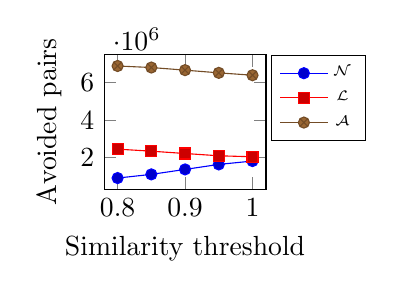
\begin{tikzpicture}
		\begin{axis}[
		scale=0.30,
		legend style={legend pos=outer north east,font=\tiny},
		xlabel=Similarity threshold,
		ylabel=Avoided pairs
		]
		\addplot coordinates { %N
			(0.8,920116)(0.85,1115817) (0.9,1380322) (0.95,1645758) (1.0,1825318) 
		};
		\addplot coordinates { %L
			(0.8,2459941)(0.85,2350823) (0.9,2227265) (0.95,2106097) (1.0,2052808) 
		};
		\addplot coordinates { %A
			(0.8,6887603)(0.85,6806034) (0.9,6666249) (0.95,6522071) (1.0,6395815) 
		};
		%\addplot coordinates { %N+L+A
		%	(0.8,1000877)(0.85,1001497) (0.9,1001633) (0.95,1001641) %(1.0,1001641) 
		%};
		%\addplot coordinates { %GoodPairs
		%	(0.8,765)(0.85,145) (0.9,9) (0.95,1) (1.0,1) 
		%};
		\legend{
			$\mathcal{N}$,
			$\mathcal{L}$,
			$\mathcal{A}$,
			$\mathcal{N}+\mathcal{L}+\mathcal{A}$,
			$GoodPairs$
			}
		\end{axis}
		\end{tikzpicture}
		\label{fig:avoided}
	}
	\subfigure[Recall.]
	{
		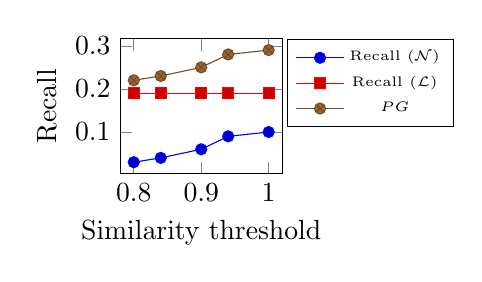
\begin{tikzpicture}
		\begin{axis}[
		scale=0.30,
		legend style={legend pos=outer north east,font=\tiny},
		xlabel=Similarity threshold,
		ylabel=Recall
		]
		\addplot coordinates { %N
			(0.8,0.03)(0.84,0.04) (0.9,0.06) (0.94,0.09) (1.0,0.10) 
		};
		\addplot coordinates { %L
			(0.8,0.19)(0.84,0.19) (0.9,0.19) (0.94,0.19) (1.0,0.19) 
		};
		\addplot coordinates { %PG
			(0.8,0.22)(0.84,0.23) (0.9,0.25) (0.94,0.28) (1.0,0.29) 
		};
		\legend{
			Recall ($\mathcal{N}$),
			Recall ($\mathcal{L}$),
			$PG$
			}		
			\end{axis}
		\end{tikzpicture}
		\label{fig:recall}
	}
	\caption{Avoided pairs and recall.}
	\label{fig:avoided2}
\end{figure}	

\subsection{Parallel implementation} \label{sec:parallel}

Our algorithm contains parallel code snippets with which we perform a load and balance of the data among CPU/GPU cores when available.
% This specific characteristic offers the possibility for utilization when the hardware is available for parallel computing, such as CPU/GPU processors.
To illustrate this part of our idea, we can state: Given a two datasets $S,T$, that contains all the strings to be compared. Thus, make a Cartesian product of the strings $S \times T$, where each pair is the processed separately in threads that are spread among CPU/GPU cores. Thus, we process the each comparison in parallel.
The parallel implementation works better in large datasets with size more than $10^5$, that was more than one time faster than the approach without parallelism and two times faster than the naive approach as shown in figures \ref{fig:a}, \ref{fig:b} and \ref{fig:c}.

\subsection{Runtime Evaluation}

% We evaluate the runtime of all filter combinations with 1,001,642 and 10,273,950 pairs of labels from DBpedia and LinkedGeodata, as can be observed in figure \ref{fig:a,fig:b}.
The evaluation in figures \ref{fig:a} and \ref{fig:b} shows that all filter setup outperform the naive approach, and the parallel approach does not suffer significant changes related to the runtime according to the size of the dataset, as show figure \ref{fig:c}.
%For the dataset with size greater than $10^3$, using a threshold %$\theta=0.92$ the runtime was increased.
%With a dataset size of 1,001,642, the best runtime average is the combination of filters $(\mathcal{L}+\mathcal{A})$ and the best runtime is 1973 milliseconds with the threshold $\theta=0.8$, see \Cref{tab.runtime}.
The experiments related to the variance of $k$, also were considered, as show in figure \ref{fig:d}, the runtime varies according the size of $k$, indicating the influence of $k$ with values from $1$ to $120$ with $1,001,642$ comparisons.
% \begin{table}[H]
% 	\caption{Time in milliseconds - $|D_s \times D_t|=1,001,642$  pairs from DBpedia and Linked Geo Data.}
% 	\centering
% 	\begin{tabular}{l|l|l|l|l|l}
% 		\hline\noalign{\smallskip}
% 		\textbf{$\theta$} & \textbf{Naive} & \textbf{($\mathcal{N}+\mathcal{L}+\mathcal{A}$)} & \textbf{(L+A)} & \textbf{($\mathcal{N}+\mathcal{A}$)} & \textbf{($\mathcal{A}$)} 
% 		\\
% 		\noalign{\smallskip}
% 		\hline
% 		\noalign{\smallskip}
% 		\textbf{0.8} & 3401 & 2077 & 1973 & 2053 & 2024 \\ 
% 		\textbf{0.85} & 3438 & 2273 & 2038 & 2112 & 2055 \\ 
% 		\textbf{0.9} & 3333 & 2273 & 2088 & 2071 & 2040 \\ 
% 		\textbf{0.95} & 3451 & 2241 & 2047 & 2054 & 2049 \\ 
% 		\textbf{1} & 3333 & 2243 & 2002 & 2000 & 2015 \\
% 		\textbf{Avg} & 3391.2 & 2221.4 & 2029.6 & 2058 & 2036.6 \\ \hline
% 	\end{tabular}
% 	\label{tab.runtime}
% \end{table}
The performance (run-time) was improved as shown in figures  \ref{fig:a}, \ref{fig:b} and according the recall with a performance gain of $26.07 \%$ as shown in figure \ref{fig:avoided2}. The time complexity is based on two sort process O(n log n) + O(m log m) resulting in O(n log n) as a upper bound in the worst case.

%\subsubsection{Time complexity}
%In order to get the time complexity of our MFKC firstly is considered the maximum frequent K characters from a string, the first step is sorting the string in a lexiconical manner. Then we can reach a linear complexity after this sort, because the input with highest occurrence can be achieved with a linear time complexity. The first string can be sorted in O (n log n) and second string on O(m log m) times like some classical sorting algorithms such as merge sort \cite{goldstine1948planning} and quick sort \cite{hoare1962quicksort} that are working in O(n log n) complexity. Thus the total complexity is O(n log n) + O(m log m) resulting in O(n log n) as a upper bound in the worst case.

\subsection{Scalability Evaluation}

In the experiments (see figures \ref{fig:c}, \ref{fig:e} and \ref{fig:f}), we looked at the growth of the runtime of our approach on datasets of growing sizes.
The results show that the combination of filters $(\mathcal{N}+\mathcal{L}+\mathcal{A})$ is the best option for datasets of large sizes.
This result holds on both DBpedia and LinkedGeoData, so our approach can be used on large datasets and achieves acceptable run-times. 
We also can realize the quantity of avoided pairs in each combination of filters in figure \ref{fig:avoided2}, that consequently brings a performance gain.
We looked at experiments with runtime behavior on a large dataset with more than $10^6$ labels as shown in figure \ref{fig:b}. The results suggest that the runtime decreases according to the threshold $\theta$ increment. Thus, one more point showing that our approach is useful on large datasets, where can be used with high threshold values for link discovery area.
About our parallel implementation, figure \ref{fig:c} shows that our GPU parallel implementation works better on large datasets with size greater than $10^5$. 
%Also we have the CPU experiments as shown in figure \ref{fig:e,fig:f}.

\subsection{Comparison with existing approaches} \label{comparisons}

Our work overcomes the naive approach \cite{seker2014novel}, thus, in order to show some important points we compare our work not only with the state of the art, but with popular algorithms such as Jaccard Index \cite{jaccard1912distribution}.
%According to \cite{seker2014novel}, the naive approach already overcomes the Levenshtein distance \cite{levenshtein1966binary} and Jaccard Index \cite{jaccard1912distribution}.
As shown in figures \ref{fig:c}, \ref{fig:e} and \ref{fig:f}, our approach outperforms not only the naive approach, but also Jaccard Index. We show that the threshold $\theta$ and $k$ have a significant influence related to the runtime.
The naive approach present some points to consider, among them, even if the naive approach states that they did experiments with k=7, the naive algorithm was designed for only k=2, there are some cases where $k=2$ is not enough to get the similarity level expected, i.e. $s=mystring1$ and $t=mystring2$ limiting $k=2$, we will have $\sigma_2(s,t)=0.2$, showing that the similarity is very low, but when $k=8$, the similarity is $\sigma_8(s,t)=0.8$ showing that sometimes we can lose a good similarity case limiting $k=2$.
Our work fix all these problems and also has a better runtime, as show figure \ref{fig:a}, figure \ref{fig:b} and figure \ref{fig:c}.

%In order to summarize main differences between the naive and our approach, also  you can see the table \ref{tab:diff}.

% Please add the following required packages to your document preamble:
% \usepackage{graphicx}
% \begin{table}[H]
% 	\caption{Main differences}
% 	\centering
% 	\begin{tabular}{l|l|l}
% 		\hline\noalign{\smallskip}
		
% 		\textbf{Main differences} & \textbf{Naive} & \textbf{Our approach}
		
% 		\\
% 		\noalign{\smallskip}
% 		\hline
% 		\noalign{\smallskip}
		
% 		Size of $k$ & maximum 2 & no limit \\ 
% 		Run-time $>10^7$ comparisons & 27594 & 16916 \\ 
% 		Similarity threshold $\theta$ & \xmark{} & \checkmark{} \\
% 		Parallel & \xmark{} & \checkmark{} \\ 
% 		Document similarity & \xmark{} & \checkmark{} \\
% 		\hline
% 	\end{tabular}%
% 	\label{tab:diff}
% \end{table}

\begin{filecontents*}{f-score.csv}
theta,MFKC,Jaccard,Jaro
0.5,0.004,0.757,0.006
0.55,0.006,0.761,0.012
0.6,0.009,0.764,0.029
0.65,0.014,0.760,0.070
0.7,0.028,0.760,0.145
0.75,0.065,0.762,0.251
0.8,0.184,0.763,0.424
0.85,0.480,0.763,0.670
0.9,0.706,0.765,0.770
0.95,0.756,0.766,0.754
1,0.752,0.770,0.770
\end{filecontents*}
\begin{filecontents*}{precision.csv}
theta,MFKC,Jaccard,Jaro
0.5,0.002,0.807,0.003
0.55,0.003,0.853,0.006
0.6,0.004,0.874,0.015
0.65,0.007,0.882,0.037
0.7,0.014,0.897,0.079
0.75,0.034,0.919,0.146
0.8,0.105,0.944,0.282
0.85,0.357,0.969,0.585
0.9,0.720,0.980,0.848
0.95,0.888,0.984,0.888
1,0.939,0.998,0.998
\end{filecontents*}
\begin{filecontents*}{recall.csv}
theta,MFKC,Jaccard,Jaro
0.5,0.961,0.713,0.952
0.55,0.935,0.687,0.933
0.6,0.911,0.678,0.922
0.65,0.882,0.667,0.910
0.7,0.838,0.660,0.902
0.75,0.806,0.651,0.884
0.8,0.775,0.640,0.855
0.85,0.731,0.629,0.785
0.9,0.693,0.627,0.705
0.95,0.658,0.627,0.655
1,0.627,0.627,0.627
\end{filecontents*}

\begin{figure}[htpb]
	\centering
	\subfigure[y axis = F-score.]
	{
		\begin{tikzpicture}
		\begin{axis}[
		scale=0.40,
		legend pos=outer north east,
		xlabel=Similarity threshold,
		%ylabel=f-score
		]
		reverse legend, legend pos=outer north east,xlabel=Trend,
    ylabel=Data]
\addplot table [x=theta, y=MFKC, col sep=comma] {f-score.csv};
\addplot table [x=theta, y=Jaccard, col sep=comma] {f-score.csv};
\addplot table [x=theta, y=Jaro, col sep=comma] {f-score.csv};
		%\legend{$MFKC$,$Jaccard$,$JaroWinker$}
		\end{axis}
		\end{tikzpicture}
		\label{fig:f-score}
	}
	\subfigure[y axis = Precision.]
	{
		\begin{tikzpicture}
		\begin{axis}[
		scale=0.40,
		legend pos=outer north east,
		xlabel=Similarity threshold,
		%ylabel=Precision
		]
		reverse legend, legend pos=outer north east,xlabel=Trend,
    ylabel=Data]
\addplot table [x=theta, y=MFKC, col sep=comma] {precision.csv};
\addplot table [x=theta, y=Jaccard, col sep=comma] {precision.csv};
\addplot table [x=theta, y=Jaro, col sep=comma] {precision.csv};
		%\legend{$MFKC$,$Jaccard$,$JaroWinker$}
		\end{axis}
		\end{tikzpicture}
		\label{fig:precision}
	}
	\subfigure[y axis = Recall.]
	{
		\begin{tikzpicture}
		\begin{axis}[
		scale=0.40,
		%legend pos=outer north east,
		legend style={at={(0.4,-1)},
                anchor=north,legend columns=-1},
		xlabel=Similarity threshold,
		%ylabel=Recall
		]
		reverse legend, legend pos=outer north east,xlabel=Trend,
    ylabel=Data]
\addplot table [x=theta, y=MFKC, col sep=comma] {recall.csv};
\addplot table [x=theta, y=Jaccard, col sep=comma] {recall.csv};
\addplot table [x=theta, y=Jaro, col sep=comma] {recall.csv};
		%\legend{$MFKC$,$Jaccard$,$JaroWinker$}
		\end{axis}
		\end{tikzpicture}
		\label{fig:recall}
	}
	\subfigure[]
	{
		\begin{tikzpicture}
		\begin{axis}[
		scale=0.000000001,
		%legend pos=outer north east,
		legend style={at={(0.4,-1)},
                anchor=north,legend columns=-1}
		]
\addplot table [x=theta, y=MFKC, col sep=comma] {recall.csv};
\addplot table [x=theta, y=Jaccard, col sep=comma] {recall.csv};
\addplot table [x=theta, y=Jaro, col sep=comma] {recall.csv};
		\legend{$MFKC$,$Jaccard$,$JaroWinker$}
		\end{axis}
		\end{tikzpicture}
	}
	\label{fig:measures}
	\caption{Precision, Recall and F-Measure.}
\end{figure}


An experiment with labels from DBpedia and Yago\footnote{\url{http://www.mpi-inf.mpg.de/departments/databases-and-information-systems/research/yago-naga/yago/}} shows that the f-score indicates a significant potential to be used with success as a string similarity comparing with Jaccard Index and Jaro Winkler, as figures \ref{fig:f-score}, \ref{fig:precision} and \ref{fig:recall} shows.
To summarize the key features that makes our approach outperform the naive approach are the following: We use more than two $K$ most frequent characters in our evaluation, our run-time for more than $10^7$ comparisons is shorter (27,594 against 16,916) milliseconds, we do have a similarity threshold, allowing us to discard comparisons avoiding extra processing, and a parallel implementation, making our approach scalable.
Jaccard does not show significant changes varying the threshold, MFKC and Jaro Winkler present a very similar increase of the f-score varying the threshold.


% \subsubsection{Document similarity}
% The difference at this point is that the MFKC algorithm can also be used to compute the similarity of documents.
% Since our algorithm is able to obtain a similarity score according to the most frequent K characters, this paradigm can be extended as follows.
% Given two text documents $d_1=$\textit{``Today I went to shop''} and $d_2=$\textit{``Yesterday the shop was open''} belonging to a collection $D$, we map all words\footnote{Without stop words.} to characters.
% For $d_1$ and $d_2$, words \textit{(today, go, shop)} and \textit{(yesterday, shop, be, open)} are mapped to characters $(1,2,3)$ and $(4,3,5,6)$ respectively.
% Applying the MFKC algorithm to strings \texttt{123} and \texttt{4356} means to find the overlap between documents w.r.t. the most used words.
% Thus, in this example, the MFKC similarity would yield a value of [INSERT-VALUE], as the the word \textit{shop} appears in both documents.
% Our filtering algorithm can therefore be used to tackle the similarity join problem in Information Retrieval systems.

\begin{figure}[H]
	\subfigure[Runtime 1,001,642 comparisons.]
	{
		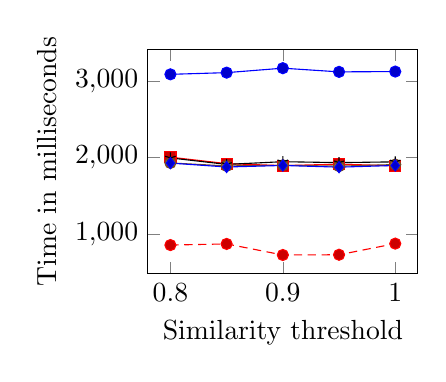
\begin{tikzpicture}
		\begin{axis}[
		scale=0.50,
		legend pos=outer north east,
		xlabel=Similarity threshold,
		ylabel=Time in milliseconds
		]
		\addplot coordinates {
			(0.8,3084)(0.85,3106) (0.9,3164) (0.95,3116) (1.0,3120) 
		};
		\addplot coordinates {
			(0.8,2006)(0.85,1922) (0.9,1896) (0.95,1915) (1.0,1894) 
		};
		\addplot coordinates {
			(0.8,1931)(0.85,1892) (0.9,1901) (0.95,1889) (1.0,1910) 
		};
		\addplot coordinates {
			(0.8,1996)(0.85,1912) (0.9,1947) (0.95,1935) (1.0,1945) 
		};
		\addplot coordinates {
			(0.8,1929)(0.85,1878) (0.9,1898) (0.95,1876) (1.0,1898) 
		};
		\addplot coordinates {
			(0.8,862)(0.85,877) (0.9,733) (0.95,736) (1.0,881) 
		};
		%\legend{$naive$,$\mathcal{L}+\mathcal{N}+\mathcal{A}$,$d=3$,$d=4$,$d=5$,$d=6$}
		\end{axis}
		\end{tikzpicture}
		\label{fig:a}
	}
	\subfigure[Runtime 10,273,950 comparisons.]
	{
		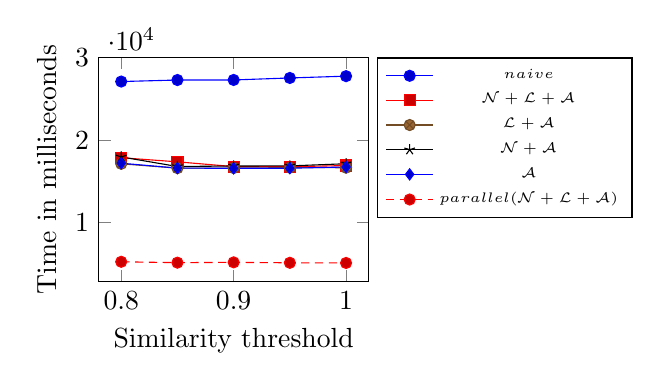
\begin{tikzpicture}
		\begin{axis}[
		scale=0.50,
		legend style={legend pos=outer north east,font=\tiny},
		xlabel=Similarity threshold,
		ylabel=Time in milliseconds
		]
		\addplot coordinates {
			(0.8,27107)(0.85,27292) (0.9,27301) (0.95,27542) (1.0,27761) 
		};
		\addplot coordinates {
			(0.8,17867)(0.85,17367) (0.9,16790) (0.95,16775) (1.0,16917) 
		};
		\addplot coordinates {
			(0.8,17128)(0.85,16600) (0.9,16611) (0.95,16664) (1.0,16655) 
		};
		\addplot coordinates {
			(0.8,17963)(0.85,16800) (0.9,16864) (0.95,16875) (1.0,17137) 
		};
		\addplot coordinates {
			(0.8,17201)(0.85,16609) (0.9,16582) (0.95,16595) (1.0,16743) 
		};
		\addplot coordinates {
			(0.8,5243)(0.85,5138) (0.9,5175) (0.95,5122) (1.0,5102) 
		};
		\legend{$naive$,
			$\mathcal{N}+\mathcal{L}+\mathcal{A}$,
			$\mathcal{L}+\mathcal{A}$,
			$\mathcal{N}+\mathcal{A}$,
			$\mathcal{A}$,
			$parallel(\mathcal{N}+\mathcal{L}+\mathcal{A})$}
		\end{axis}
		\end{tikzpicture}
		\label{fig:b}
	}
	\subfigure[The parallel approach improves the performance for more than $10^5 comparisons$.]
	{
		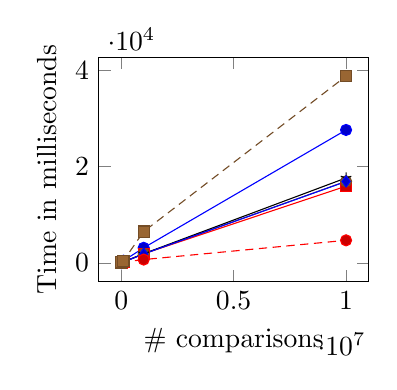
\begin{tikzpicture}
		\begin{axis}[
		scale=0.50,
		legend style={legend pos=outer north east,font=\tiny},
		xlabel=\# comparisons,
		ylabel=Time in milliseconds
		]
		\addplot coordinates {
			(1000,40)(10000,113) (100000,464) (1000000,3144) (10000000,27594) 
		};
		\addplot coordinates {
			(1000,13)(10000,63) (100000,226) (1000000,1913) (10000000,15932) 
		};
		\addplot coordinates {
			(1000,9)(10000,43) (100000,208) (1000000,1889) (10000000,16935)  
		};
		\addplot coordinates {
			(1000,6)(10000,36) (100000,208) (1000000,1925) (10000000,17638)  
		};
		\addplot coordinates {
			(1000,5)(10000,32) (100000,192) (1000000,1875) (10000000,16916) 
		};
		\addplot coordinates { %parallel
			(1000,70)(10000,86) (100000,171) (1000000,708) (10000000,4700)  
		};
		%\addplot coordinates { %JaroWinkler
		%	(1000,7)(10000,28) (100000,133) (1000000,898) (10000000,7716)  
		%};
		\addplot coordinates { %Jaccard
			(1000,38)(10000,153) (100000,475) (1000000,6516) (10000000,38755)  
		};
		%\legend{$naive$,$\mathcal{L}+\mathcal{N}+\mathcal{A}$,$d=3$,$d=4$,$d=5$,$d=6$}
		\end{axis}
		\end{tikzpicture}
		\label{fig:c}
	}
	\subfigure[Runtime $k$ most frequent characters, with values of $k$ from $1$ to $120$, over $1,001,642$ comparisons, $\theta=0.95$.]
	{
		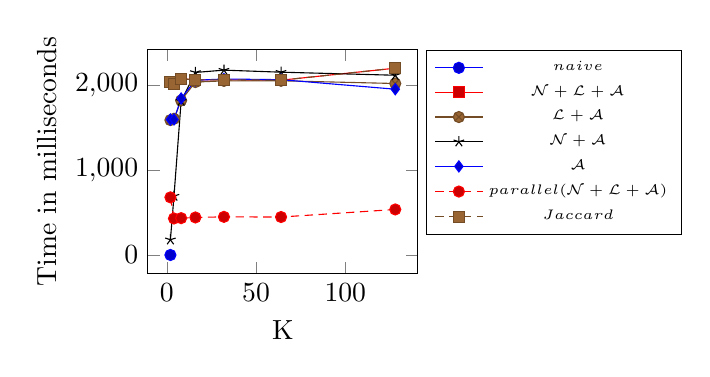
\begin{tikzpicture}
		\begin{axis}[
		scale=0.50,
		legend style={legend pos=outer north east,font=\tiny},
		xlabel=K,
		ylabel=Time in milliseconds
		]
		\addplot coordinates {
			(2,00)
		};
		\addplot coordinates {
			(2,2028)(4,2012) (8,2072) (16,2057) (32,2058) (64,2054) (128,2195)
		};
		\addplot coordinates {
			(2,1585)(4,1600) (8,1816) (16,2032) (32,2046) (64,2047) (128,2015)
		};
		\addplot coordinates {
			(2,179)(4,692) (8,1807) (16,2145) (32,2172) (64,2148) (128,2112)
		};
		\addplot coordinates {
			(2,1592)(4,1593) (8,1839) (16,2053) (32,2068) (64,2060) (128,1948)
		};
		\addplot coordinates { %parallel
			(2,677)(4,429) (8,433) (16,441) (32,448) (64,446) (128,535)
		};
		%\addplot coordinates {
		%	(2,2028)(4,2012) (8,2072) (16,2057) (32,2058) (64,2054) (128,2195)
		%};
		\addplot coordinates {
			(2,2028)(4,2012) (8,2072) (16,2057) (32,2058) (64,2054) (128,2195)
		};
		\legend{$naive$,
			$\mathcal{N}+\mathcal{L}+\mathcal{A}$,
			$\mathcal{L}+\mathcal{A}$,
			$\mathcal{N}+\mathcal{A}$,
			$\mathcal{A}$,
			$parallel(\mathcal{N}+\mathcal{L}+\mathcal{A})$,
			%$JaroWinkler$,
			$Jaccard$}
		\end{axis}
		\end{tikzpicture}
		\label{fig:d}
	}
	\subfigure[CPU Speedup of algorithm ($1,001,642$ comparisons).]
	{
		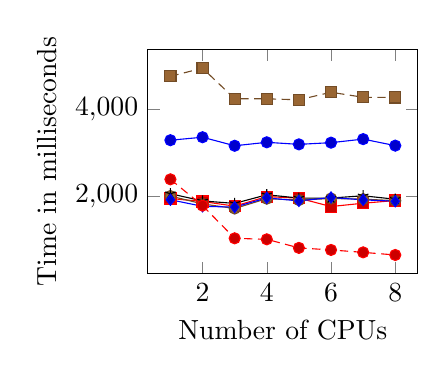
\begin{tikzpicture}
		\begin{axis}[
		scale=0.50,
		legend style={legend pos=outer north east,font=\tiny},
		xlabel=Number of CPUs,
		ylabel=Time in milliseconds
		]
		\addplot coordinates {
			(1,3292) (2,3360) (3,3165) (4,3244) (5,3197) (6,3236) (7,3317) (8,3168) 
		};
		\addplot coordinates {
			(1,1960) (2,1891) (3,1785) (4,2003) (5,1967) (6,1776) (7,1852) (8,1913) 
		};
		\addplot coordinates {
			(1,2016) (2,1836) (3,1731) (4,1956) (5,1924) (6,1960) (7,1945) (8,1911)  
		};
		\addplot coordinates {
			(1,2069) (2,1904) (3,1848) (4,2045) (5,1970) (6,1970) (7,2022) (8,1943)   
		};
		\addplot coordinates {
			(1,1931) (2,1781) (3,1763) (4,1974) (5,1905) (6,1983) (7,1929) (8,1897)  
		};
		\addplot coordinates { %Parallel
			(1,2398) (2,1798) (3,1050) (4,1027) (5,831) (6,784) (7,729) (8,669)   
		};
		%\addplot coordinates { %JaroWinkler
		%	(1,1027) (2,968) (3,898) (4,925) (5,905) (6,935) (7,907) (8,905)   
		%};
		\addplot coordinates { %Jaccard
			(1,4752) (2,4938) (3,4240) (4,4238) (5,4215) (6,4388) (7,4273) (8,4270)   
		};
		%\legend{$naive$,$\mathcal{L}+\mathcal{N}+\mathcal{A}$,$d=3$,$d=4$,$d=5$,$d=6$}
		\end{axis}
		\end{tikzpicture}
		\label{fig:e}
	}
	\subfigure[CPU Speedup of algorithm ($10,273,950$ comparisons).]
	{
		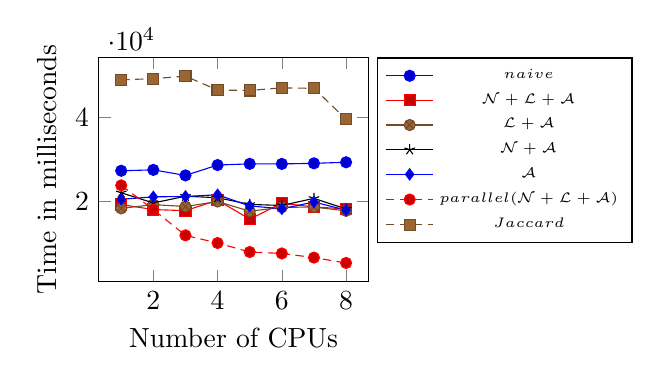
\begin{tikzpicture}
		\begin{axis}[
		scale=0.50,
		legend style={legend pos=outer north east,font=\tiny},
		xlabel=Number of CPUs,
		ylabel=Time in milliseconds
		]
		\addplot coordinates { %naive
			(1,27308) (2,27520) (3,26196) (4,28672) (5,28958) (6,28943) (7,29085) (8,29336) 
		};
		\addplot coordinates { %(N+L+A)
			(1,19218) (2,18025) (3,17764) (4,20261) (5,15740) (6,19538) (7,18650) (8,18178) 
		};
		\addplot coordinates { %(L+A)
			(1,18306) (2,19202) (3,18758) (4,19948) (5,17629) (6,18562) (7,18617) (8,17708)  
		};
		\addplot coordinates { %(N+A)
			(1,22037) (2,19602) (3,21217) (4,20860) (5,19257) (6,19004) (7,20703) (8,18159)   
		};
		\addplot coordinates { %(A)
			(1,20479) (2,21062) (3,21157) (4,21564) (5,18894) (6,18208) (7,19830) (8,17884)  
		};
		\addplot coordinates { %(Parallel)
			(1,23810) (2,18005) (3,11855) (4,10018) (5,7871) (6,7524) (7,6529) (8,5249)   
		};
		%\addplot coordinates { %(JaroWinkler)
		%	(1,10496) (2,9805) (3,10491) (4,9849) (5,9965) (6,9937) (7,10145) (8,8982)   
		%};
		\addplot coordinates { %(Jaccard)
			(1,49062) (2,49339) (3,49938) (4,46605) (5,46523) (6,47134) (7,47029) (8,39611)   
		};
		\legend{$naive$,
			$\mathcal{N}+\mathcal{L}+\mathcal{A}$,
			$\mathcal{L}+\mathcal{A}$,
			$\mathcal{N}+\mathcal{A}$,
			$\mathcal{A}$,
			$parallel(\mathcal{N}+\mathcal{L}+\mathcal{A})$,
			%$JaroWinkler$,
			$Jaccard$}
		\end{axis}
		\end{tikzpicture}
		\label{fig:f}
	}
	
	\caption{Run-time experiments results.}
	\label{fig:results}
\end{figure}

%\begin{figure}
%    \subfigure[Precision according to the threshold $\theta$]
%    {
%        \includegraphics[width=\textwidth]{img/precision1}
%        \label{fig:f}
%    }
%    \caption{Results.}
%    \label{fig:results2}
%\end{figure}

%\section{Conclusion and Future work} \label{conclusion}